% =======================================================================================
% MODELO DE TCC - INSTITUTO FEDERAL DE SERGIPE (IFS)
% =======================================================================================
% Autores do Modelo (discentes de Ciência da Computação - IFS, Campus Itabaiana):
%   Mikael dos Santos Gois
%   Talyson Rodrigues Silva Nascimento
%   Kauan Gutierrez Santos Estácio
% Modelo Base: abnTeX2, adaptado para as normativas internas de TCC do IFS (Art. 31 e 34)
% Créditos dos modelos base (abnTeX2, DECOM/UFOP e Diogo D. Moreira) e das imagens: ver NOTICE
% Licença: CC BY-SA 4.0 (ver LICENSE)
% Este arquivo faz parte de um modelo opensource para estudantes do IFS.
% Não remova os créditos dos autores originais e do modelo base.
% Este modelo é fornecido "no estado em que se encontra", sem garantias de qualquer tipo.
% =======================================================================================

% [O que aparece no PDF Bookmark] {O que aparece impresso no documento}
\chapter[Fundamentação Teórica]{FUNDAMENTAÇÃO TEÓRICA}
\label{sec:fundamentacao-teorica}

% 1. TEXTO DE ABERTURA 
A fundamentação teórica é a seção inicial de desenvolvimento do trabalho, onde os conceitos principais são apresentados e contextualizados. Nela, o autor deve expor a revisão da literatura e detalhar as tecnologias escolhidas, criando a base de conhecimento necessária para que o leitor compreenda a viabilidade do estudo. Esta seção deve ser clara, objetiva e devidamente embasada em autores reconhecidos pela comunidade científica.

Neste capítulo, serão abordados os conceitos fundamentais sobre [INSERIR TEMA 1], as características da ferramenta [INSERIR TEMA 2] e o funcionamento do [INSERIR TEMA 3].
% EXEMPLO DE SEÇÃO COM INSERÇÃO DE FIGURA 
% ------------------------------------------------------------------------------
\section{Estrutura e Arquitetura de Sistemas}

% DICA PARA O ESTUDANTE:
% Sempre referencie a figura no texto ANTES dela aparecer, usando o comando \ref{}.
Para compreender o funcionamento da solução proposta, é essencial analisar os modelos clássicos de processamento. A arquitetura computacional padrão pode ser visualizada na Figura \ref{fig:exemplo_arquitetura}. Nela estão representados todos os componentes principais de interação.

% BLOCO PADRÃO PARA INSERIR FIGURAS (ESTILO ABNT / IFS)
% Substitua o título, o caminho da imagem e a fonte pelos dados do seu TCC.
\begin{figure}[htb]
    \centering
    \caption{Título da sua ilustração (Ex: Arquitetura de Von Neumann)}
    % Ajuste a largura (width) conforme necessário e coloque o nome do seu arquivo
    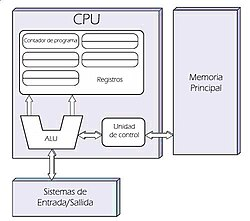
\includegraphics[width=0.7\textwidth]{figuras/Arquitecturaneumann.jpg}
    % DICA: a fonte vai logo abaixo da ilustração, com a expressão de autoria
    % (NBR 14724:2024, 5.8). Se você criou a imagem:
    %   \fonte{Elaborada pelo autor (2026).}
    % Se adaptou de outro autor: \fonte{Adaptada de \citeonline{referencia}.}
    % A imagem de EXEMPLO deste modelo é o diagrama de von Neumann de David strigoi
    % (Wikimedia Commons, domínio público) - ver NOTICE. Substitua a imagem, o
    % arquivo em figuras/ e este crédito pelos seus.
    \fonte{Imagem de exemplo: David strigoi, Wikimedia Commons (domínio público). Adaptada de \citeonline{tanenbaum2013}.}
    \label{fig:exemplo_arquitetura}
\end{figure}

Como apresentado no fluxo da imagem anterior, [AQUI O ESTUDANTE DEVE EXPLICAR COM SUAS PALAVRAS O QUE A IMAGEM SIGNIFICA E COMO ELA SE APLICA AO SEU CONTEXTO].

%Ex Subseções
\subsection{O Paradigma do Processamento em PCs}

Exemplo de subseção, ou seção secundária.

%Ex: Subsubseções
\subsubsection{Limitações da Abordagem Baseada em PC}

Exemplo de seção terciária.